\documentclass[12pt,a4paper]{jsarticle}
\usepackage[dvipdfmx]{graphicx}
\usepackage[dvipdfmx]{color}
\usepackage{listings,jlisting}% to use japanese correctly, install jlistings.
\lstset{
  basicstyle={\ttfamily},
  identifierstyle={},
  commentstyle={\color{red}},
  keywordstyle={\bfseries\color{cyan}},
  ndkeywordstyle={},
  stringstyle={\color{blue}},
  frame={tb},
  breaklines=true,
  numbers=left,
  numberstyle={},
  stepnumber=1,
  numbersep=1zw,
  xrightmargin=0zw,
  xleftmargin=3zw,
  lineskip=0.5ex
}
\lstdefinestyle{customCsh}{
  language={csh},
  numbers=none,
}
\lstdefinestyle{customRuby}{
  language={ruby},
  numbers=left,
}
\lstdefinestyle{customTex}{
  language={tex},
  numbers=none,
}
\lstdefinestyle{customJava}{
  language={java},
  numbers=left,
}
\begin{document}
\title{卒業論文\\
\vspace{4cm} ユーザメモソフトmy\_helpのビヘイビアテスト開発}
\author{ 関西学院大学 理工学部 情報科学科\\\\2535 那須比呂貴}
\date{\vspace{3cm} 2017年  3月\\
\vspace{3cm} 指導教員  西谷 滋人 教授}
\maketitle
\setcounter{tocdepth}{4}
\tableofcontents

\begin{itemize}
\item \verb|{{attach_anchor(my_help_nasu.pdf,my_help_nasu)}}|
\end{itemize}
 本研究ではユーザメモソフトであるmy\_helpの開発において,BDDを取り入れることによりmy\_helpの向上を目指した.

 my\_helpとは,ユーザメモソフトであり,user独自のhelpを作成・提供することができるgemである.
しかし,これらの仕様方法を初心者が理解すること自体に時間がかかってしまうという問題点がある.
そこで,cucumberを用いる.cucumberはRubyでBDDを実践するために用意された環境である.
したがって,cucumberは振る舞いをチェックするために記述するが,そこで日本語がそのまま用いることが可能であるため,その記述を読むだけで,my\_helpの振る舞いを理解することが可能となる.

 cucumberは実際にソフトウェア開発の現場において,ユーザーとプログラマがお互いの意思疎通のために利用される.
テストはプログラムがチェックしてくれるが,記述は人間が理解できなければならない.
この二つの要求を同時に叶えようというのが,BDDの基本思想である.
これらは,研究室の知識を定着させることに有益であり,研究室の役に立つと考えた.


\section{序論}
プログラム開発では,統合開発環境がいくつも用意されているが,多くの現場では,terminal上での開発が一般的です.
ところが,プログラミング初心者はterminal上でのcharacter user interface(CUI)を苦手としています.
プログラミングのレベルが上がるに従って,shell commandやfile directory操作, process制御にCUIを使うことが常識です.

この不可欠なCUIスキルの習得を助けるソフトとして,ユーザメモソフトmy\_helpがruby gemsに置かれています.
このcommand line interface(CLI)で動作するソフトは,helpをterminal上で簡単に提示するものです.
また,初心者が自ら編集することによって,すぐに参照できるメモとしての機能を提供しています.
これによって,terminal上でちょっとした調べ物ができるため,作業や思考が中断することなく
プログラム開発に集中できること,さらに初心者のスキル習得が加速することが期待できます.

しかし,Ruby gemsとして提供されているこのソフトは,動作はしますがテストが用意されていません.
熟練した開発者は,テストを見ることで仕様を理解するのが常識です.
今後ソフトを進化させるために共同開発を進めていくには,仕様や動作の標準となるテスト記述が不可欠となります.

そこで,本研究では,ユーザメモソフトであるmy\_helpのテストを開発することを目的とします.
本研究では、テスト駆動開発の中でも,ソフトの振る舞いを記述します.
ビヘイビア駆動開発(Behavior Driven Development:BDD)に基づいてテストを記述していきます.
Rubyにおいて、BDD環境を提供する標準的なフレームワークであるCucumberとRSpecを用いて,
my\_helpがどのような振る舞いをするのかを記述します.
Cucumberは自然言語で振る舞いを記述することができるため,開発者や,ユーザにとっても,わかりやすく振る舞いを確認することができます.


\section{先行研究,方法}
ここでは、本研究で使用するcucumberの特徴について詳述する.
cucumberはビヘイビア駆動開発(bdd)を実現するフレームワークである.
まずはbddの現れた背景や現状を示した後、Cucumberの記述の具体例を示して,
その特徴を詳述する.
さらに,本研究の対象となるmy\_helpの振る舞いを使用法とともに示す.


\subsection{RSpecとBDDについて}
ビヘイビア駆動開発(Behaviour-Driven Development : BDD)は,テスト駆動開発(Test-Driven Development : TDD)の工程への理解を深め,それをうまく説明しようとして始まりました.TDDの持つ単語のイメージが構造のテストを中心とするべしというのに対して,BDDはソフトの振る舞いに中心をおきなさいという意図があります.この違いが,初めに考えるべきテストの性質を変化させ,構造ではなく振る舞いを中心にテストを構築するという意識をもたせてくれます.

さらに,ソフトの中で,オブジェクト同士がコミュニケーションをとるように,実世界において開発チームやテストチーム,あるいはドキュメントチーム間のコミュニケーションの取り方をシステムで提供しようというのがBDDのフレームワークです.CucumberとRSpecはこれを実現する一つのシステムとして提供されています.

RSpecとCucumberの関係を図\ref{fig:001}に示しました.これは,RSpec本から書き写した図です[1, pp.9].RSpecでテストを書くと一つ一つのfunctionあるいはmethodレベルでRed, Green, Refactoringを行うべしという意図があります.一方で,もっと大きな枠組み,つまりシステムレベルでもこれらのステップは必要です.ところが,それをRSpecで書くのには無理があります.このレベルのテスト記述をしやすくするのが,Cucumberです.そこでもRed, Green, Refactoringが必要で,そこでサイクルが回ることを意図しています.

\begin{figure}[htbp]\begin{center}
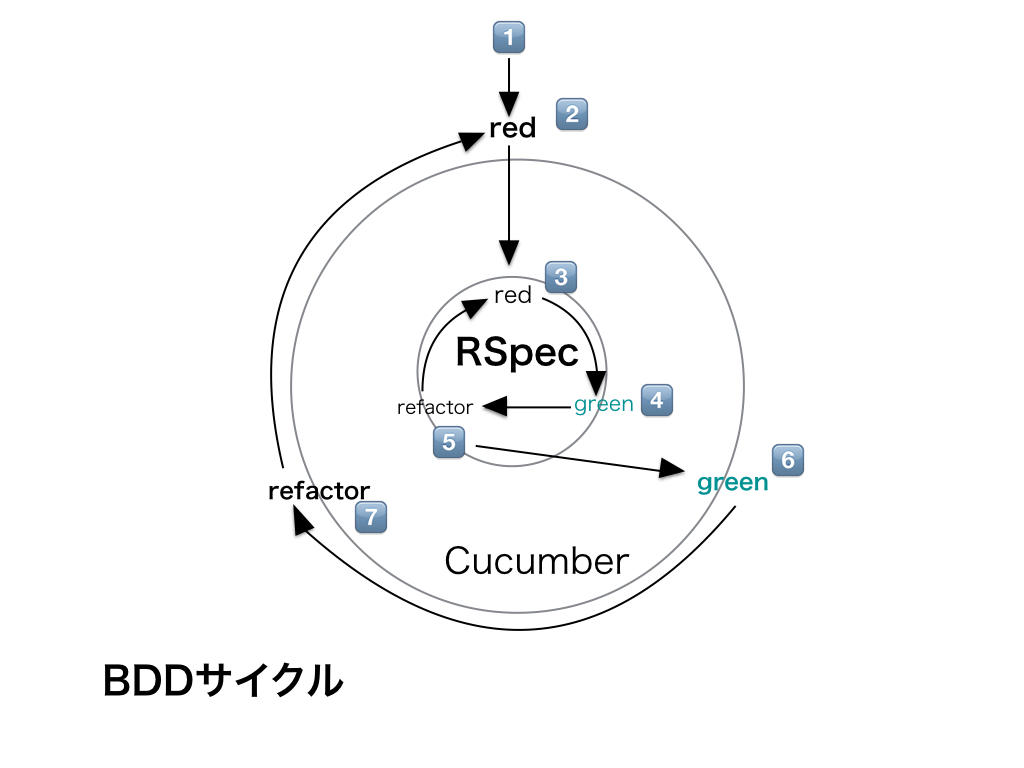
\includegraphics[width=12cm,bb= 0 0 937 753]{../figs/./my_help_nasu.001.jpeg}
\caption{RSpecとCucumberのRed-Green-Refactoringサイクル間の関係.}
\label{fig:001}
\label{default}\end{center}\end{figure}
BDDの基本的な考え方は次の通りまとめられています.

\begin{quotation}
BDDの目的は,ソフトウェアが使われる状況を説明するための言語を単純化することで,ソフトウェア開発チームのコミュニケーションを後押しすることです.つまり,あるコンテキストで(Given),あるイベントが発生すると(When),ある結果が期待されます(Then).BDDにおけるGiven, When, Thenの3つの単語は,アプリケーションやオブジェクトを,それらの振る舞いに関係なく表現するために使われる単純な単語です.ビジネスアナリスト,テスト担当者,開発者は皆,それらをすぐに理解します.これらの単語はCucumberの言語に直接埋め込まれています[1, pp.3-6].

\end{quotation}
手順を書き直すと図\ref{fig:002}の通りです.

\begin{figure}[htbp]\begin{center}
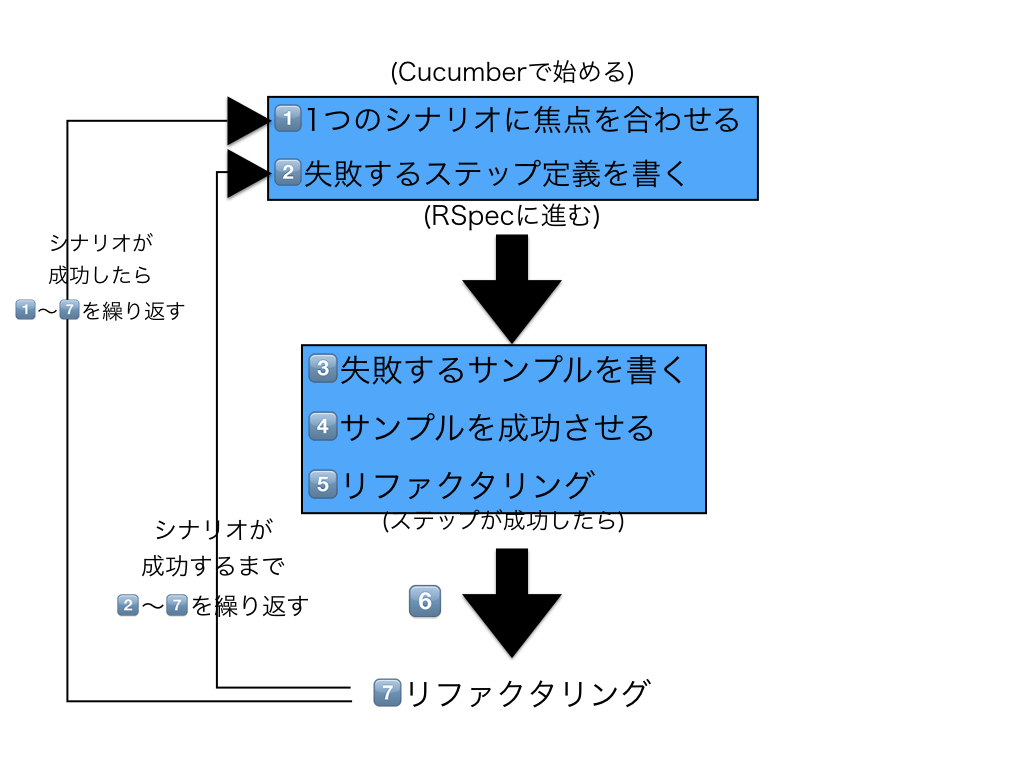
\includegraphics[width=12cm,bb= 0 0 937 753]{../figs/./my_help_nasu.002.jpeg}
\caption{RSpecとCucumberの手順.}
\label{fig:002}
\label{default}\end{center}\end{figure}
まずCucumberで一つのシナリオに焦点を当てて,その振る舞いを記述するfeatureを書きます.一つずつつぶしていくのがこつです.一つのfeatureが書けたら、次に,それぞれfeatureを実現するステップに分けて仕様を決めて行きます.これはTDDのred green refactoringの前に行う作業,「仕様をきめる」に対応しています.このプロセスが終了したら,RSpecに行きます.
RSpecでは実際にテストコードを書き,ここでもred, green, refactoringを行います.
RSpecが成功したら,Cucumberのrefactoringを行います.



\subsection{Cucumberについて}
\subsubsection{概要}
Cucumberが提供するBDDの内容をまとめると

\begin{quotation}
BDDはフルスタックのアジャイル開発技法です.BDDはATDP(Acceptance Test-Driven Planning)と呼ばれるAcceptance TDDの一種を含め,エクストリームプログラミングからヒントを得ています.ATDPでは,顧客受け入れテストを導入し,それを主体にコードの開発を進めて行きます.それらは顧客と開発チームによる共同作業の結果であることが理想的です.開発チームによってテストが書かれた後,顧客がレビューと承認を行うこともあります.いずれにしても,それらのテストは顧客と向き合うものなので,顧客が理解できる言語とフォーマットで表現されていなければなりません.Cucumberを利用すれば,そのための言語とフォーマットを手に入れることができます.Cucumberは,アプリケーションの機能とサンプルシナリオを説明するテキストを読み取り,そのシナリオの手順に従って開発中のコードとのやり取りを自動化します[1, 7pp.].

\end{quotation}
と記されている.

\subsubsection{features}
Cucumberでは先の引用にある通り、振る舞いをシナリオとしてまず記述します.
シナリオとは,一つひとつの振る舞いを,主にGiven(前提), Then(もし), When(ならば)に分けてfeaturesを記述します.
次に,英語のfeaturesのひな形を示します.
\begin{lstlisting}[style=customRuby,basicstyle={\scriptsize\ttfamily}]
% cat ./featrues/sample_e.feature
Feature: Description of feature

Scenario: Description of scenario
  Given I want to explain scenario
  Then I investigate
  When I know the meaning
\end{lstlisting}
ファイルの先頭で,
\begin{quote}\begin{verbatim}
# language: ja
\end{verbatim}\end{quote}
と記すと日本語でのkeywordが認識されます.下記にmy\_todoに対するfeaturesファイルの具体例を示します.
\begin{lstlisting}[style=customCsh,basicstyle={\scriptsize\ttfamily}]
# language: ja

機能: todoの更新を行う
自分のするべきことを書き込むためにtodoを更新する

シナリオ: コマンドを入力してtodoを更新していく
 前提   todoを編集したい
 もし   "my_todo --edit"と入力する
 ならば editが開かれる
 かつ   自分のtodoを書き込む
\end{lstlisting}
このようにFeature, Scenario, Given, Then, Whenなどのcucumberが解釈する大文字で始まる
keywordsに対して,それぞれ機能,シナリオ,前提,もし,ならばなどの単語があてられています.
この機能により,より自然な日本語でfeaturesを書くことができ,
顧客にもわかりやすく,開発者も書きやすくなっています。

featureファイルで用意されているkeywordは
\begin{quote}\begin{verbatim}
cucumber --i18n LANG
\end{verbatim}\end{quote}
によって表示される.LANG=ja, enに対しては表\ref{table:one}の通りになっています.

\begin{table}[htbp]\begin{center}
\caption{featureファイルで用意されているkeywordの日本語(ja),英語(en)の対応表.}
\label{table:one}
\begin{tabular}{llll}
\hline
keyword   &ja(japanese)   &en(english)  \\ \hline
 feature  & "フィーチャ", "機能"      &"Feature", "Business Need",   \\
 & &"Ability"     \\
background  &"背景"  &"Background"   \\
scenario  &"シナリオ"        &"Scenario"     \\
 scenario\_outline   &"シナリオアウトライン",  &"Scenario Outline",  \\
 &"シナリオテンプレート","テンプレ",  & "Scenario Template"   \\
 &"シナリオテンプレ"   & \\
examples  &"例", "サンプル"   &"Examples", "Scenarios"          \\
given   &"* ", "前提"        &"* ", "Given "          \\
when   &"* ", "もし"        &"* ", "When "  \\
then   &"* ", "ならば"       &"* ", "Then "  \\
and    &"* ", "かつ"        &"* ", "And "   \\
but    &"* ", "しかし", "但し", "ただし"  &"* ", "But "   \\
given (code)   &"前提"   &"Given"        \\
when (code)   &"もし"     &"When"         \\
then (code)   &"ならば"   &"Then"         \\
and (code)    &"かつ"     &"And"          \\
but (code)    &"しかし", "但し","ただし"   &"But"          \\
\hline
\end{tabular}
\label{default}
\end{center}\end{table}
%for inserting separate lines, use \hline, \cline{2-3} etc.

\subsubsection{Cucumber,RSpecインストール}
まずrspecをgemでinstallする.

\begin{enumerate}
\item gem install rspec --version 2.0.0
\item rspec --help
\end{enumerate}
と入力して
\begin{lstlisting}[style=customCsh,basicstyle={\scriptsize\ttfamily}]
/Users/nasubi/nasu% rspec --help
Usage: rspec [options] [files or directories]
\end{lstlisting}
のような表示がされていればinstallができている.次に,cucumberをinstallする

\begin{enumerate}
\item gem install cucumber --version 0.9.2
\item cucumber --help
\end{enumerate}
と入力して
\begin{lstlisting}[style=customCsh,basicstyle={\scriptsize\ttfamily}]
cucumber --help
Usage: cucumber [options] [ [FILE|DIR|URL][:LINE[:LINE]*] ]+
\end{lstlisting}
のような表示がされていればinstallできている.

\subsubsection{ディレクトリー構造と使用手順}
cucumberはRubygemsの提供する基本directory構造での作業を前提としています.
その構造を表示すると次のようになります.
\begin{quote}\begin{verbatim}
bob% tree .
.
├── Gemfile
├── Rakefile
├── features
│   ├── hogehoge.feature
│   ├── step_definitions
│   │   └── hogehoge_step.rb
│   ├── support
│       ├── env.rb
├── lib
│   ├── daddygongon
│   │   ├── emacs_help.yml
│   │   ├── my_todo.yml
├── pkg
├── spec
│   ├── my_help_spec.rb
│   ├── my_todo
│   │   ├── todo_spec.rb
│   ├── spec_helper.rb
│   └── support
│       └── aruba.rb
\end{verbatim}\end{quote}
カレントディレクトリ(.)の中にfeaturesというサブディレクトリを作成します.
そのfeaturesの中に書きたいシナリオを書いた,hogehoge.featureを作成します.
featureの具体例は上記に示してします.

次にシェルを開いて,カレントディレクトリで,
\begin{quote}\begin{verbatim}
cucumber features hogehoge.feature
\end{verbatim}\end{quote}
と入力します.そうすると以下のような出力が得られます.
\begin{lstlisting}[style=customRuby,basicstyle={\scriptsize\ttfamily}]
Feature: Description of feature

  Scenario: Description of scenario  # features/hogehoge.feature:3
    Given I want to explain scenario # features/hogehoge.feature:4
    Then I investigate      # features/hogehoge.feature:5
    When I know the meaning # features/hogehoge.feature:6

1 scenario (1 undefined)
3 steps (3 undefined)
0m0.066s

You can implement step definitions for undefined steps with these snippets:

Given(/^I want to explain scenario$/) do
  pending # Write code here that turns the phrase above into concrete actions
end

Then(/^I investigate$/) do
  pending # Write code here that turns the phrase above into concrete actions
end

When(/^I know the meaning$/) do
  pending # Write code here that turns the phrase above into concrete actions
end

\end{lstlisting}
ここではステップ定義に使用することができるコードブロックが表示されています.
ステップ定義はステップを作成するための方法です.このサンプルでは,Giver(), When(), Then()の
3つのメソッドを使ってステップを記述します.
これらのメソッドはそれぞれ\/\/で囲まれたRegexp(正規表現)とブロックを受け取ります.
Cucumberはシナリオの最初のステップを読み取り,そのステップにマッチする正規表現を持つステップ定義を探します.
その中の対応するステップ定義のブロックを実行します.

これはfeaturesディレクトリの下にstep\_definitionsディレクトリーにあることになっています.
このシナリオを成功させるには,Cucumberが読み込めるファイルにステップ定義を保存する必要があります[1, pp15.].
その内容は次の通りcucumberから自動生成されます.
\begin{lstlisting}[style=customRuby,basicstyle={\scriptsize\ttfamily}]

Given(/^I want to explain scenario$/) do
  pending # Write code here that turns the phrase above into concrete actio\
ns  
end

Then(/^I investigate$/) do
  pending # Write code here that turns the phrase above into concrete actio\
ns  
end

When(/^I know the meaning$/) do
  pending # Write code here that turns the phrase above into concrete actio\
ns  
end

\end{lstlisting}
pendingを削除して,そこにあれば良いなと思うコードを記述していきます.
ここまでがCucumberの使用方法のテンプレートです.



\subsection{my\_helpについて}
my\_helpは本研究室の西谷が開発したものです.
my\_helpとはユーザメモソフトであり,CUIスキルの習得を助けてくれます.
tarminal上で簡単に提示させることができるため,プログラミングに集中することができるといった特徴があります.
また,自分の見やすいように初心者でも簡単に編集することができ,すぐに参照できるメモとしても使うことができます.

\subsubsection{my\_helpの開発動機と特徴}
以下はmy\_helpのREADMEからの抜粋です[2].

\paragraph{概要}
my\_help - CUI(CLI)ヘルプのUsage出力を真似て,user独自のhelpを作成・提供するgem.

\paragraph{開発動機}
CUIやshell, 何かのプログラミング言語などを習得しようとする初心者は,
commandや文法を覚えるのに苦労します.少しのkey(とっかかり)があると
思い出すんですが,うろ覚えでは間違えて路頭に迷います.問題点は,

\begin{itemize}
\item manは基本的に英語
\item manualでは重たい
\item いつもおなじことをwebで検索して
\item 同じとこ見ている
\item memoしても,どこへ置いたか忘れる
\end{itemize}
などです.

\paragraph{特徴}
これらをgem環境として提供しようというのが,このgemの目的です.
仕様としては,

\begin{itemize}
\item userが自分にあったmanを作成
\item 雛形を提供
\begin{itemize}
\item おなじformat, looks, 操作, 階層構造
\end{itemize}
\item すぐに手が届く
\item それらを追加・修正・削除できる
\end{itemize}
hikiでやろうとしていることの半分くらいはこのあたりのことなの
かもしれません.memoソフトでは,検索が必要となりますが,my\_helpは
key(記憶のとっかかり)を提供することが目的です.

\subsubsection{my\_helpのインストール}
githubに行ってdaddygongonのmy\_helpをforkします.

\begin{enumerate}
\item git clone git@github.com:daddygongon/my\_help.git
\item cd my\_help
\item rake to\_yml
\item rake clean\_exe
\item [sudo] bundle exec exe/my\_help -m
\item source ~/.zshrc or source ~/.cshrc
\item my\_help -l
\item rake add\_yml
\end{enumerate}
\subsubsection{my\_helpの更新}
git hubを用いてmy\_helpを新しくします.

\begin{enumerate}
\item git remote -vをする(remoteの確認).
\item (upstreamがなければ)git remote add upstream git@github.com:gitname/my\_help.git
\item git add -A
\item git commit -m 'hogehoge'
\item git push upstream master(ここで自分のmy\_helpをupstreamに送っとく)
\item git pull origin master(新しいmy\_helpを取ってくる)
\end{enumerate}
次にとってきた.ymlを~/.my\_helpにcpする.

\begin{enumerate}
\item cd my\_helpでmy\_helpに移動.
\item cp hogehoge.yml ~/.my\_help
\end{enumerate}
それを動かすために
(sudo)bundle exec ruby exe/my\_help -mをする.
ここで過去にsudoをした人はpermissionがrootになっているので,sudoをつけないとerrorが出ます.
(sudoで実行していたら権限がrootに移行される)

\begin{enumerate}
\item 新しいターミナルを開いて動くかチェックする.
\end{enumerate}


\section{ビヘイビア駆動開発の実践}
CucumberとRSpecを用いてBDDでmy\_helpのテスト開発を進めて行きました.
ビヘイビア駆動開発のコツとして「焦点を合わせる」ことが強調されています.
ここでは,焦点を合わせたmy\_helpの中での一つの振る舞いである
「todoの更新」を例として詳しく見て行きます.

\subsection{todoの更新マニュアル}
最初に,todoを更新するときの手順を示します.

\begin{enumerate}
\item my\_todo --editを入力して~/.my\_help/my\_todo.ymlを開く
\item editorでtodoを書き込む(今週やることならweeklyというitemを作ってそこに書き込む)
\item 保存して~/.my\_help/my\_todo.ymlを閉じる
\end{enumerate}
この振る舞いがきちんとできているのかをBDDでテストを書いていきます.

\subsection{Cucumber}
以下はtodoの更新を行うときのfeatureです.
まず,適当なディレクトリにfeaturesというディレクトリを作成します.
次に先ほど作成した,featuresディレクトリにmy\_todo.featureを作成します.
\begin{lstlisting}[style=customCsh]
# language: ja 

機能: todoの更新を行う
自分のするべきことを書き込むためにtodoを更新する

 シナリオ: コマンドを入力してtodoを更新していく
          前提 todoを編集したい
          もし "my_todo --edit"と入力する
          ならば editが開かれる
          かつ 自分のtodoを書き込む
\end{lstlisting}
機能とは,このシステムの機能のことを記述します.ここでは,todoを更新するシステムですので,「todoの更新を行う」です.
機能の下には,機能の補足説明を記述します.機能の補足説明では,ルールがないので自分がわかりやすいように,記述するのが常識です.
シナリオは,その名の通りtodoを更新する時のユーザの行動やシステム振る舞いを前提,もし,ならば,かつ,しかしに分類して記述します.

ここまでfeatureが記述できたら,次はcucumberコマンドを実行してみます.
コマンドは以下の通りです.
\begin{quote}\begin{verbatim}
nasu% cucumber features/my_todo.feature
\end{verbatim}\end{quote}
featuresディレクトリにあるmy\_todo.featureファイルをcucumberで実行するという意味です.

実行すると図\ref{cucumber01}のようになります.

\subsubsection{caption:(fig:cucumber01)step定義をする前のcucumberの実行結果.}
\begin{figure}[htbp]\begin{center}
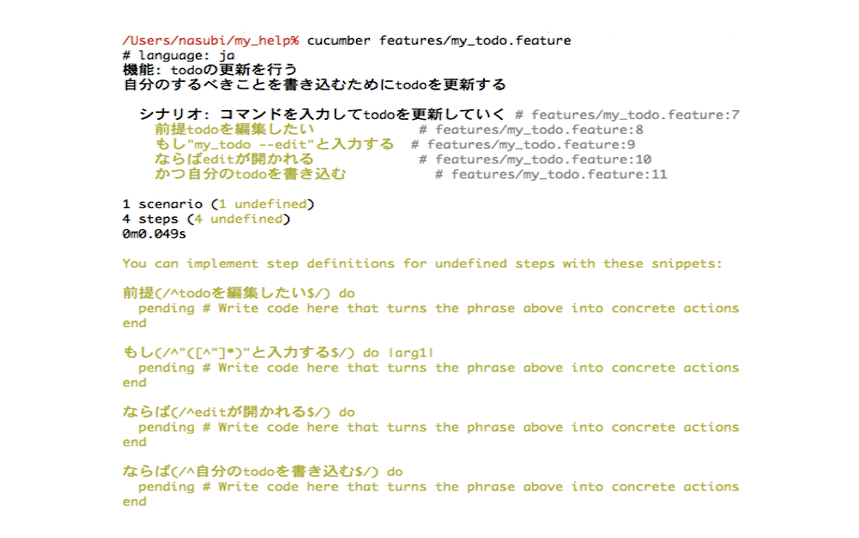
\includegraphics[width=10cm,bb= 0 0 737 553]{../figs/./cucumber01.001.jpg}
\caption{}
\label{default}\end{center}\end{figure}
ここでは,1つのscenarioと4つのstepが失敗しています.
まだstep定義を記述していないので当たり前です.

一度cucumberを実行したのには理由があります.
featureを書いた時点でcucumberを実行すると,ステップ定義の元となるコマンドを,cucumberが自動的に作成してくれるからです.

以下がcucumberから出力されたステップ定義の元となる部分です.
\begin{lstlisting}[style=customCsh]
前提(/^todoを編集したい$/) do

end

もし(/^"([^"]*)"と入力する$/) do |command|

end

ならば(/^editが開かれる$/) do
  
end

ならば(/^自分のtodoを書き込む$/) do

end
\end{lstlisting}
これをコピーして,featuresディレクトリの中でstep\_definitionsディレクトリを作成し,その中にmy\_todo\_spec.rbを作成し,そこに貼付けます.

ここでもう一度cucumberを実行してみると図\ref{cucumber02}のように変化が出てきます.

\subsubsection{caption:(fig:cucumber02)defaultのstep定義を貼り付けた後のcucumberの実行結果.}
\begin{figure}[htbp]\begin{center}
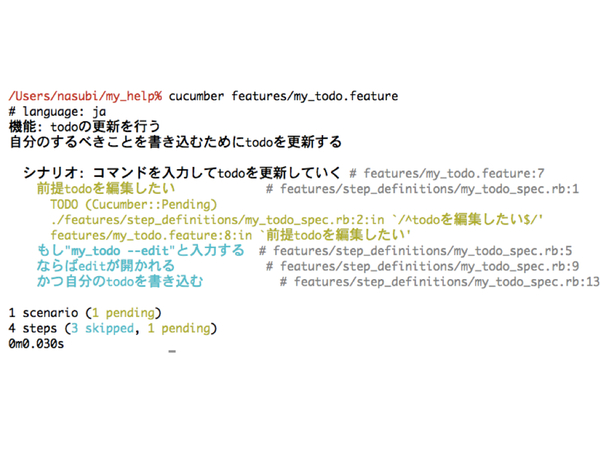
\includegraphics[width=10cm,bb= 0 0 737 553]{../figs/./cucumber02.001.jpg}
\caption{}
\label{default}\end{center}\end{figure}\begin{quote}\begin{verbatim}
1 scenarios (1 pending)
4 steps (3 skipped, 1 pending)
\end{verbatim}\end{quote}
これは1つのシナリオがあり,1つがpendingであり,4つのstepの内1つがpendingで3つがskipしたことを表しています.
step\_definitionsのmy\_todo\_spec.rbのpending部分を書き換えて,step\_definitionsの記述を進めて行きます.

まず,「前提」を見てみるとmy\_helpが何か振る舞いをすることはありません.
よって,このままにしておきます.
「もし」もユーザが入力するコマンドであり,my\_helpが何か振る舞いをすることはないのでこのままにしておきます.
次に,「ならば」を見てみるとmy\_helpがeditを開くという振る舞いをしています.
ステップ定義では,あれば良いと思うコードを記述するので私は下記のように記述しました.
\begin{lstlisting}[style=customCsh]
ならば(/^editが開かれる$/) do
  Mytodo::Edit.new.open
end
\end{lstlisting}
pendingの部分が書けたので,もう一度cucumber features/my\_todo.featureを実行します.
すると,図\ref{fig:cucumber03}のような結果が返ってきました.

\subsubsection{caption:(fig:cucumber03)pendingのstep定義を書き込んだ後のcucumberの実行結果.}
\begin{figure}[htbp]\begin{center}
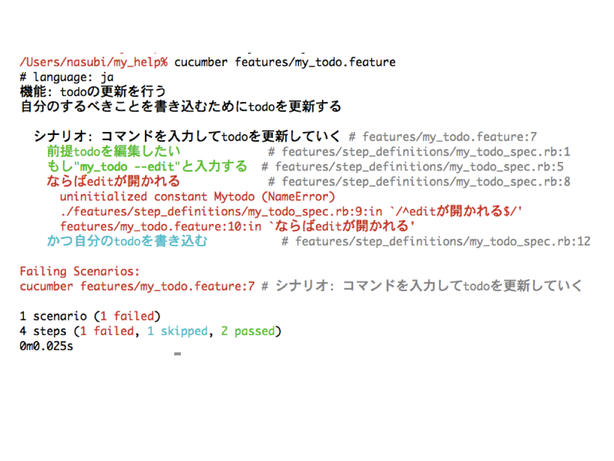
\includegraphics[width=10cm,bb= 0 0 737 553]{../figs/./cucumber03.001.jpg}
\caption{}
\label{default}\end{center}\end{figure}
Cucumberは,エラーが出たステップのすぐ後ろにエラーを表示してくれます.
ここでCucumberでエラーが出たので,この「ならば editが開かれる」のシナリオに注目してRSpecに進むことにします.

\subsection{RSpec}
次にRSpecを使って実際にtodoを更新する振る舞いをするコード書いていきます.

そのための準備として,まずspecというディレクトリを作成し,my\_todoというサブディレクトリを追加します.
次に,このサブディレクトリにtodo\_spec.rbというファイルを追加します.
作業を進める過程で,lib/my\_todo/my\_todo.rbソースファイルとspec/my\_todo/todo\_spec.rbスペックファイルが1対1に対応するといった要領で,
並列のディレクトリ構造を築いていきます.
この機能はmy\_help --editと入力されれば,~/.my\_help/my\_todo.ymlが開かれるのでその振る舞いをするコードを書きます.
まずtodo\_spec.rbは下記の通りになります.
\begin{lstlisting}[style=customRuby]
require 'spec_helper'


module Mytodo
  describe Todo do
    describe "#open" do
      it "open file my_todo.yml" 
    end
  end
end

\end{lstlisting}
describe()メソッドは,RSpecのAPIにアクセスしてRSpec::Core::ExampleGroupのサブクラスを返します.
ExampleGroupクラスはオブジェクトに期待される振る舞いのサンプルを示すグループです.
it()メソッドはサンプルを作成します.

完成したコードを下記の通りです.
\begin{lstlisting}[style=customRuby]
require 'spec_helper'


module Mytodo
  describe Todo do
    describe "#open" do
      it "open file my_todo.yml" do
          system("emacs ~/.my_help/my_todo.yml")
      end
    end
  end
end

\end{lstlisting}
specディレクトリのmy\_todoディレクトリをrspecで実行すると下記のような結果がでました.
\verb|--color|を付け加えるとわかりやすく色づけをしてくれて,見やすくなります.

\subsubsection{caption:(fig:cucumber04)pendingのstep定義を書き込んだ後のcucumberの実行結果.}
\begin{figure}[htbp]\begin{center}
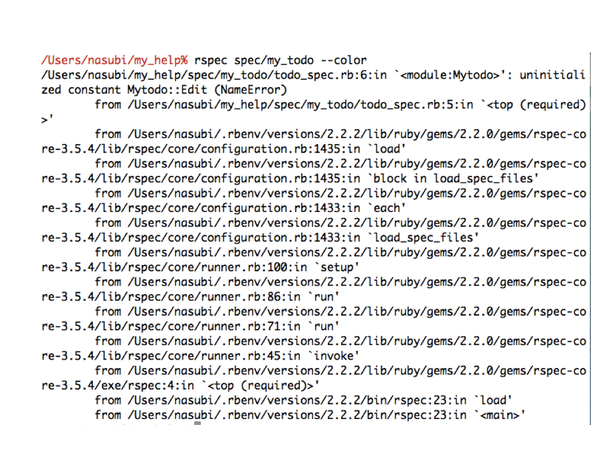
\includegraphics[width=10cm,bb= 0 0 737 553]{../figs/./cucumber04.001.jpg}
\caption{}
\label{default}\end{center}\end{figure}
図\ref{fig:cucumber04}を見るとエラーが出てしまっているのがわかります.
\begin{quote}\begin{verbatim}
`<module:Mytodo>': uninitialized constant Mytodo::Edit (NameError)
\end{verbatim}\end{quote}
上記のエラーを解決するために,specディレクトリの一つ上の構造のディレクトリにlibディレクトリを作成します.
その中にmy\_todoというディレクトリを作成し,my\_todo.rbを作成します.

構造を表示すると以下のようになっています.
\begin{quote}\begin{verbatim}
/Users/nasubi/my_help/lib/my_todo% ls
my_todo.rb
\end{verbatim}\end{quote}
my\_todo.rbに先ほどのエラーでMytodoというmoduleがないといわれているので,
ここで作成します.

/Users/nasubi/my\_help/lib/my\_todo/my\_todo.rbの中に以下のコードを記述します.
\begin{lstlisting}[style=customCsh]
module Mytodo
  class Edit
    def open

    end
  end
end
\end{lstlisting}
また,これをrequireしないといけないので,lib/todo.rbとして,以下を追加します.
\begin{quote}\begin{verbatim}
require 'my_todo/my_todo'
\end{verbatim}\end{quote}
これだけでは,rspecがlib/my\_todo/my\_todo.rbを読み込んでいないため,このスペックを実行するために,specディレクトリにspec\_helper.rbに以下を追加します.
\begin{lstlisting}[style=customCsh]
$LOAD_PATH.unshift File.expand_path('../../lib', __FILE__)
require 'todo'
\end{lstlisting}
これでもう一度rspecを実行してみます.

\subsubsection{caption:(fig:rspec01)redを修正してgreenになったrspecの実行結果}
\begin{figure}[htbp]\begin{center}
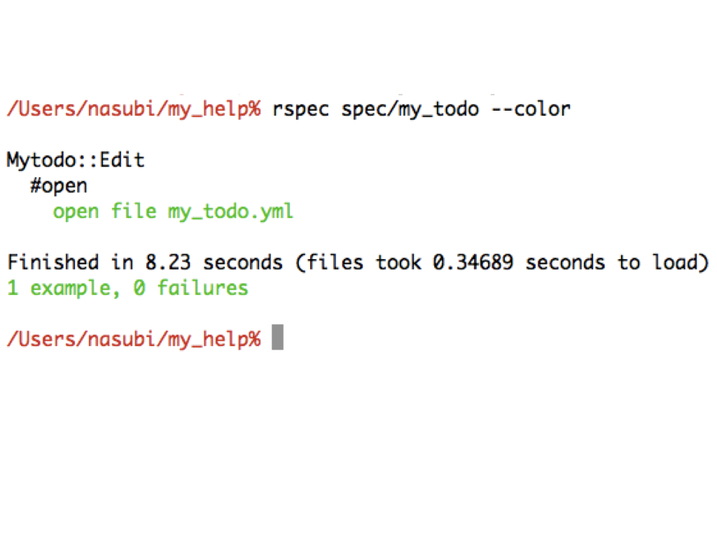
\includegraphics[width=10cm,bb= 0 0 737 553]{../figs/./rspec01.001.jpg}
\caption{}
\label{default}\end{center}\end{figure}
エラーが消えて成功しているのがわかります.
これで「ならば editが開かれる」のシナリオのRSpec部分が成功しました.
Red, Greenと進めたので次はRefactoringをするのですが,ここではあまり必要のないので省略します.
RSpecが終わったので,Cucumberに戻ります.

先ほどlibディレクトリでlib/my\_todo/my\_todo.rbを作成したので,cucumberでも読み込むために,以下を作成します.
\begin{quote}\begin{verbatim}
/Users/nasubi/my_help/features/support/env.rb
\end{verbatim}\end{quote}
env.rbの中は以下の通りです.
\begin{lstlisting}[style=customRuby]
$LOAD_PATH.unshift File.expand_path('../../../lib', __FILE__)
require 'todo'
\end{lstlisting}
これでcucumberもlib/の中身を読み取ってくれます.

もう一度cucumberを実行してみると,

\subsubsection{caption:(fig:cucumber05)libの中身を読み込むようにしたcucumberの実行結果.}
\begin{figure}[htbp]\begin{center}
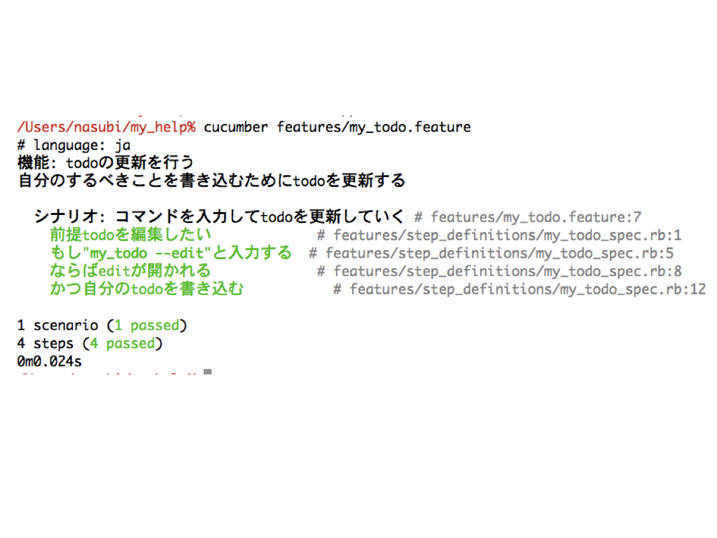
\includegraphics[width=10cm,bb= 0 0 737 553]{../figs/./cucumber05.001.jpg}
\caption{}
\label{default}\end{center}\end{figure}
エラーが消えています.

これでBDDが成功しました.
残りの「自分のtodoを書き込む」もmy\_helpが何か振る舞いをするわけではないので,「コマンドを入力してtodoを更新する」シナリオ全てのテスト開発が終わりました.
このようにBDDでmy\_helpのテスト開発を行っていきました.



\subsection{featuresでの記述とその意味}
featuresでの記述は,コマンドの振る舞いを説明する自然な記述です.
その様子をspecific\_helpが用意しているデフォルトのコマンドについて説明します.
specific\_helpとは,ユーザが作成するそれぞれのヘルプです.
speific\_helpの--helpを表示させると,
\begin{lstlisting}[style=customCsh,basicstyle={\scriptsize\ttfamily}]
        --edit                       edit help contentsを開く
        --to_hiki                    hikiのformatに変更する
        --all                        すべてのhelp画面を表示させる
        --store [item]               store [item] でback upをとる
        --remove [item]              remove [item] back upしてるlistを消去する
        --add [item]                 add new [item]で新しいhelpを作る
        --backup_list [val]          back upしているlistを表示させる
\end{lstlisting}
が得られます.
これらの項目について順に詳細な振る舞いとそれを記述するシナリオを検討していきます.

\subsubsection{--add [item]}
このコマンドは新しいitemをspecific\_helpに追加します.
提供される機能をシナリオの先頭に内容をかいつまんでこの振る舞いが記述されています.
実装では,ヘルプの内容は~/.my\_help/emacs\_help.ymlに元dataがあります.
\begin{lstlisting}[style=customRuby,basicstyle={\scriptsize\ttfamily}]
nasu% cat add.feature
#language: ja

#--add [item]
機能: 新しいitemをspecific_helpに追加する
specific_helpとは,ユーザが作成するそれぞれのヘルプである
新しいhelp画面を追加したい

シナリオ: コマンドを入力してspecific_helpにitemを追加する
        前提 新たなhelpコマンドを追加したい
        もし emacs_help --add[item]を入力する
        ならば ~/.my_help/emacs_help.ymlに新しいitemが自動的に追加される

\end{lstlisting}
\subsubsection{--all}
このコマンドはspecific\_helpにあるhelpを一度に全て表示させます.
するとspecific\_helpにあるitemを全て表示します.
実装では,元データが~/.my\_help/emacs\_help.ymlにあるので,それを全て表示します.
\begin{lstlisting}[style=customRuby,basicstyle={\scriptsize\ttfamily}]
nasu% cat all_help.feature
#language: ja

#--all
機能: 全てのhelp画面を見る
複数のhelp画面を一度に見たい時に便利である

シナリオ: コマンドを入力してすべてのhelpを見る
        前提 複数のhelp画面を表示したい
        もし emacs_help --allと入力する
        ならば すべてのhelp画面が表示される
\end{lstlisting}
\subsubsection{--backup\_list}
このコマンドは過去にバックアップをとったことのあるitemを表示させます.
自分がどのitemをバックアップしたのかの確認を行えます.
また,そのitemのバックアップをとった時間も表示されるので,いつバックアップをとったのかの確認も行えます.
\begin{lstlisting}[style=customRuby,basicstyle={\scriptsize\ttfamily}]
nasu% cat backup_list.feature
#language: ja

#--backup_list
機能: 過去にバックアップしてあるitemのリストを表示させる
何をバックアップしたかの確認をしたい

シナリオ: コマンドを入力してバックアップのリストを見る
        前提 バックアップのリストを見たい
        もし emacs_help --backup_listを入力する
        ならば バックアップしているitemのリストが表示される
        
\end{lstlisting}
\subsubsection{--edit}
このコマンドはspecific\_helpのitemの編集ができます.
実装では,元データのある~/.my\_help/emacs\_help.ymlがemacsで開かれ,自分で編集ができます.
編集作業が終了したら,emacsで開かれているので, [C-x C-s]で保存,[C-x C-c]でeditを閉じます.
\begin{lstlisting}[style=customRuby,basicstyle={\scriptsize\ttfamily}]
nasu% cat edit_help.feature
# language: ja
#--edit
機能: helpコマンドの追加や削除,編集をするためのeiditを開く
emacs_helpと入力したときに出てくるhelpのコマンドの追加や削除,編集ができる

シナリオ: コマンドを入力してeditを開く
        前提 emacs_helpのコマンドの編集がしたい
        もし emacs_help --editと入力する
        ならば ~/.my_help/emacs_help.ymlがemacsで開かれる
\end{lstlisting}
\subsubsection{--remove [item]}
このコマンドは新しいitemをspecific\_helpから削除します.
提供される機能をシナリオの先頭に内容をかいつまんでこの振る舞いが記述されています.
実装では,ヘルプの内容は~/.my\_help/emacs\_help.ymlに元dataがあります.
\begin{lstlisting}[style=customRuby,basicstyle={\scriptsize\ttfamily}]
nasu% cat remove.feature
#language: ja

#--remove [item]
機能: specific_helpのitemを消す
いらなくなったitemを消したいときに使う

シナリオ: コマンドを入力してitemを消す
        前提 いらないitemを消したい
        もし emacs_help remove [item]
        ならば ~/.my_help/emacs_help.ymlからitemが消える

\end{lstlisting}
\subsubsection{--store [item]}
このコマンドはspecific\_helpのitemのバックアップをとります.
少しhelpを新しくしたいが,過去のhelpを残しておけば安心できます.
~/.my\_helpディレクトリーの中に,同じ名前の先頭に'.'をつけたファイルに追記されていきます.
\begin{quote}\begin{verbatim}
-rw-r--r--   1 bob  501   3231  2 10 17:11 my_todo.yml
-rw-r--r--   1 bob  501  31925  2  3 19:49 .my_todo.yml
\end{verbatim}\end{quote}
などとしてます.
\begin{lstlisting}[style=customRuby,basicstyle={\scriptsize\ttfamily}]
nasu% cat store.feature
#language: ja

#--store [item]
機能: itemのバックアップを取る
バックアップとして残したいitemがあるときに使う

シナリオ: コマンドを入力してitemのバックアップをとる
        前提 バックアップをとっておきたい
        もし emacs_help --store [item]と入力する
        ならば 入力したitemのバックアップが作られる
\end{lstlisting}
\subsubsection{--to\_hiki}
このコマンドはformatをhikiに変更します.
\begin{quote}\begin{verbatim}
:カーソル移動:cursor
*C-f, move Forwrard,    前or右へ
*C-b, move Backwrard,   後or左へ
*C-a, go Ahead of line, 行頭へ
*C-e, go End of line,   行末へ
*C-n, move Next line,   次行へ
*C-p, move Previous line, 前行へ
\end{verbatim}\end{quote}
などとhiki記法で出力されます.これをhikiの本文中に入れると
\begin{description}
\item[カーソル移動] cursor

\end{description}
\begin{itemize}
\item C-f, move Forwrard,    前or右へ
\item C-b, move Backwrard,   後or左へ
\item C-a, go Ahead of line, 行頭へ
\item C-e, go End of line,   行末へ
\item C-n, move Next line,   次行へ
\item C-p, move Previous line, 前行へ
\end{itemize}
などとweb上で表示されます.
\begin{lstlisting}[style=customRuby,basicstyle={\scriptsize\ttfamily}]
nasu% cat to_hiki.feature
# language: ja

#--to_hiki
機能:formatをhikiモードに変更する
一つ一つエディタで開いて変更するのがめんどくさい時に有益である

シナリオ: コマンドを入力してformatをhikiモードに変える
        前提 hikiモードに変更したい
        もし emacs_help --to_hikiと入力する
        ならば formatがhikiモードに変更される
\end{lstlisting}
\subsubsection{todoの更新}
まず,todoを書き込むために,editを開くために,my\_todo --editと入力します.
--editコマンドは上記で説明した動きをします.
しかし,ここでは元データは~/.my\_help/todo\_help.ymlです.
editが開かれたら,todoを書き込みます.(今週やることならweeklyというitemを作ってそこに書き込む)
保存方法や,editの閉じ方はemacsと同じ操作方法です.
\begin{lstlisting}[style=customRuby,basicstyle={\scriptsize\ttfamily}]
nasu% my_todo.feature
# language: ja

機能: todoの更新を行う
自分のするべきことを書き込むためにtodoを更新する

シナリオ: コマンドを入力してtodoを更新していく
          前提 todoを編集したい
          もし "my_todo --edit"と入力する
          ならば editが開かれる
          かつ 自分のtodoを書き込む

\end{lstlisting}

\section{考察と今後の課題}
\subsection{考察}
my\_helpを対象とした具体的なビヘイビア駆動開発の実践を通して,以下のような問題点が明らかになってきました.

\subsubsection{Cucumberを記述できるようになるまで時間がかかる}
日本語で書くことができるので,記述されているコードを「理解する」のは容易で,「記述する」ことも可能であると考えていました.ところが,The RSpec Book\cite{RSpecBook}に記載されているテンプレートが少なく,理解することにも非常に困難を覚えました.自力で何も前例のない状況から作成することはできますが,やはり時間がかかってしまいます.ネットで検索しても,日本語のサイトではほぼThe RSpec Book\cite{RSpecBook}と類似したシナリオしか記載されていないのも問題の一つであり,違った種類の書き方のテンプレートがもっと必要です.地道に幾度もCucumberを叩いて,featuresやrspecの記述すること,またそのデータベースを蓄えていくことが必要です.
また,BDDではCucumberでエラーが出ている状況が正しく,Cucumberを放置してRSpecへと進みます.今までのプログラミングとは少し違う感覚に陥り,不安がよぎります.これは慣れるまでの辛抱ではありますが,この問題も時間との戦いです.

\subsubsection{BDDを行うときにrubyの知識が必要}
Cucumberのステップ定義やRSpecにおいてrubyを用いることが多々あります.スッテプ定義を記述するときに,あればよいと思うコードを書くのですが,具体的なプログラムを書くよりも難易度が高いと感じました.部分的なプログラムを作成するので,知識がないと正しいかどうかの判断が最後にしかできません.BDDを通してrubyを学べるという考え方もできますが,BDDでrubyを学ぶには物足りなさがあり,不向きです.したがって,BDDを使用する前にrubyの基礎の勉強は不可欠です.

\subsection{my\_helpの今後}
my\_helpのテスト記述が完了するに伴って,仕様や動作の標準が確定しました.
my\_helpは今後も開発者,ならびに多くのユーザの使用を通じて,どのように進化させれば便利なのかが徐々にわかってくることで,my\_helpはまだまだ進化する機会が出てくると思われます.
つまり,ビヘイビアの記述を利用することで,今後my\_helpを進化させるための共同開発が円滑に進める手助けになると推測します.
また,my\_helpの進化の開発だけに関わらず,my\_helpの使用方法が明確になったことで,本研究で作成したmy\_helpのfeaturesを読めば初心者でもmy\_helpの振る舞いが容易に理解できます.
my\_helpは本研究室で今後使われていくと予想し,本研究はこれからの研究の手助けになります.
今後の本研究室の研究生が,CUIなどの習得に時間をかけずにプログラミングに集中でき,研究の質が向上すると予想できます.


\section{謝辞}\begin{quote}\begin{verbatim}
本研究を進めるにあたり,様々なご指導を頂きました西谷滋人教授先生に深く感謝いたします.
\end{verbatim}\end{quote}
また,本研究の進行に伴い,様々な助力,知識の供給を頂きました西谷研究室の同輩,先輩方に心から感謝の意を示します.
本当にありがとうございました.

\begin{thebibliography}{99}
\bibitem{RSpecBook}   "The RSpec Book", David Chelimsky, Dave Astels, Zach Dennis, 訳, 株式会社クイーブ, 監修, 角谷信太郎, 豊田裕司 (翔泳社, 2012).
\bibitem{README}   my\_help README, Shigeot R. Nishitani, \verb|http://www.rubydoc.info/gems/my_help/0.4.3| 2017/2/11アクセス.
\end{thebibliography}
\end{document}
